\documentclass[preprintnumbers,amsmath,amssymb,twocolumn]{revtex4-1}
\usepackage{graphicx}% Include figure files
\usepackage{dcolumn}% Align table columns on decimal point
\usepackage{bm}% bold math
\usepackage{natbib}
\usepackage{physics}
\usepackage[caption=false]{subfig}

\def\sgn{\mathop{\rm sgn}}

\begin{document}

\title{Optical detection of hydrogen paramagnetic defects in diamonds}

\author{C. Pellet-Mary$^{1}$}
\author{P. Huillery $^{1}$}
\author{A. Tallaire $^{1}$...}
\author{M. Perdriat $^{1}$}
\author{G. H\'etet$^{1}$} 

\affiliation{$^1$Laboratoire de Physique de l'Ecole normale sup\'erieure, ENS, Universit\'e PSL, CNRS, Sorbonne Universit\'e, Universit\'e Paris-Diderot, Sorbonne Paris Cit\'e, Paris, France.}

\begin{abstract}
We observe cross-relaxation amongst closely packed negatively charged nitrogen-vacancy centers (NV$^-$) that involve dipolar interaction between NV centers and paramagnetic defects. 
Specifically, we observe dipolar coupling between pairs of NV$^-$ centers and between single  NV$^-$ centers and NV$^- -^{13}$C pairs as well as novel optical cross-relaxation with hydrogen-vacancy complexes.  These processes are detected using magnetic fields scans along the $\langle 100 \rangle$ cristalline direction of diamond.
Contrary the more commonly chosen $\langle 111 \rangle$ direction, $\langle 100 \rangle$ scans select dipolar couplings involving the exchange of two quanta of spin-projection.
The technique can be used to detect the degree of polarisation of $^{13}$C atoms at room temperature.
 %Scanning a magnetic field from zero to a few hundred Gauss along the $\langle 100 \rangle$ cristalline direction of diamond, we identify double-quantum cross-relaxation processes amongst NV centers. 
%In particular, the technique is shown to enable efficient micro-wave free detection of the $^{13}$C atoms on the first shell around the NV centers.centers. 
\end{abstract}
\maketitle

The precise control of the spin of negatively charged nitrogen-vacancy (NV$^-$) centers in diamond has given rise to a wealth of applications in nanoscale sensing, quantum information science etc.. 
One major reason for the interest in NV centers is that they can be optically polarized at room temperature.  
This property can be employed to manipulate and to detect other dark spins inside or outside the diamond. 

Cross relaxation.
Most of the measurements are done at the ESLAC/GLSAC. OORT, BUDKER, HOLLENBERG, BAJAJ, MANSON ? 

Polsarisation of 13C at low fields : PINES, MERILES. 
Theory GALI.
Detection at low fields was also demonstrated \cite{van_oort_optically_1991, van_oort_cross-relaxation_1989, armstrong_nvnv_2010, jarmola_longitudinal_2015, akhmedzhanov_microwave-free_2017, akhmedzhanov_magnetometry_2019, holliday_optical_1989, choi_depolarization_2017}. It was suggested that spin relaxation beyond the phonon-relaxation timescales comes from electron tunneling between nearby impurities. 
Dipolar coupling amongst closely packed NV was used further to demonstrate many body effects such as critcal thermalisation, or Dicke time crystals or beyond Heisenberg limited sensing (Lukin).
 
To the best of our knowledge, the process was however not employed to detect other impurities. 


D. SUTER.
However, 13C was not detected. The main reason is the predominance of single-quantum processes.
13C detected using B field scans ? nop. 
%Recently, this high degree of control was employed to study strongly interacting, dense NV ensembles to explore quantum many-body dynamics.
Here, we characterize the cross-relaxation of high-density NV ensembles with a focus on double quantum resonances. 

\begin{figure}[!ht]
  \centering \scalebox{0.5}{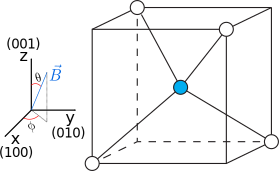
\includegraphics{Cristallo.eps}}
  \caption{a) Schematics showing the tetrahedron in one of the interstitial sites of the diamond structure. The NV centers can only be in of the four depicted orientations. 
   }\label{Cristallo}
\end{figure}

\begin{figure}[!ht]
  \centering {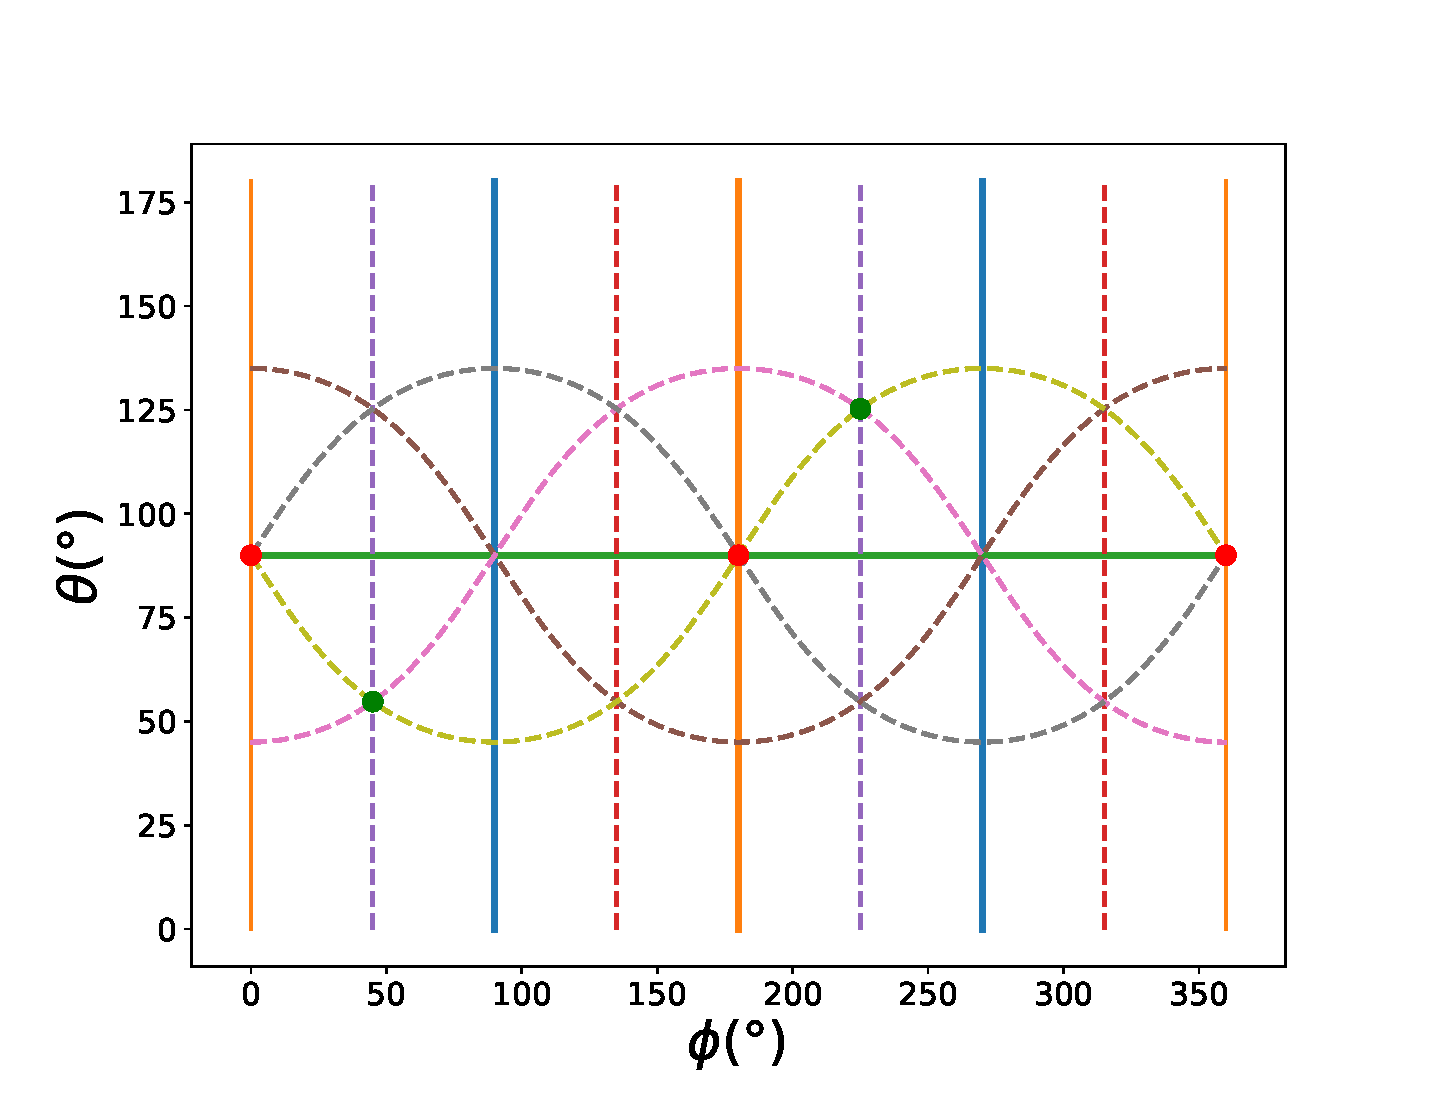
\includegraphics[width=0.4\textwidth]{map_full.eps}}
  \caption{a) 
Graph (theory) showing the locus of the degeneracies of the 4 NV centers electronic spins resonances in the $(\theta,\phi)$ parameter space. See text for details.  
 }
\end{figure}

\begin{figure}[!ht]
  \centering{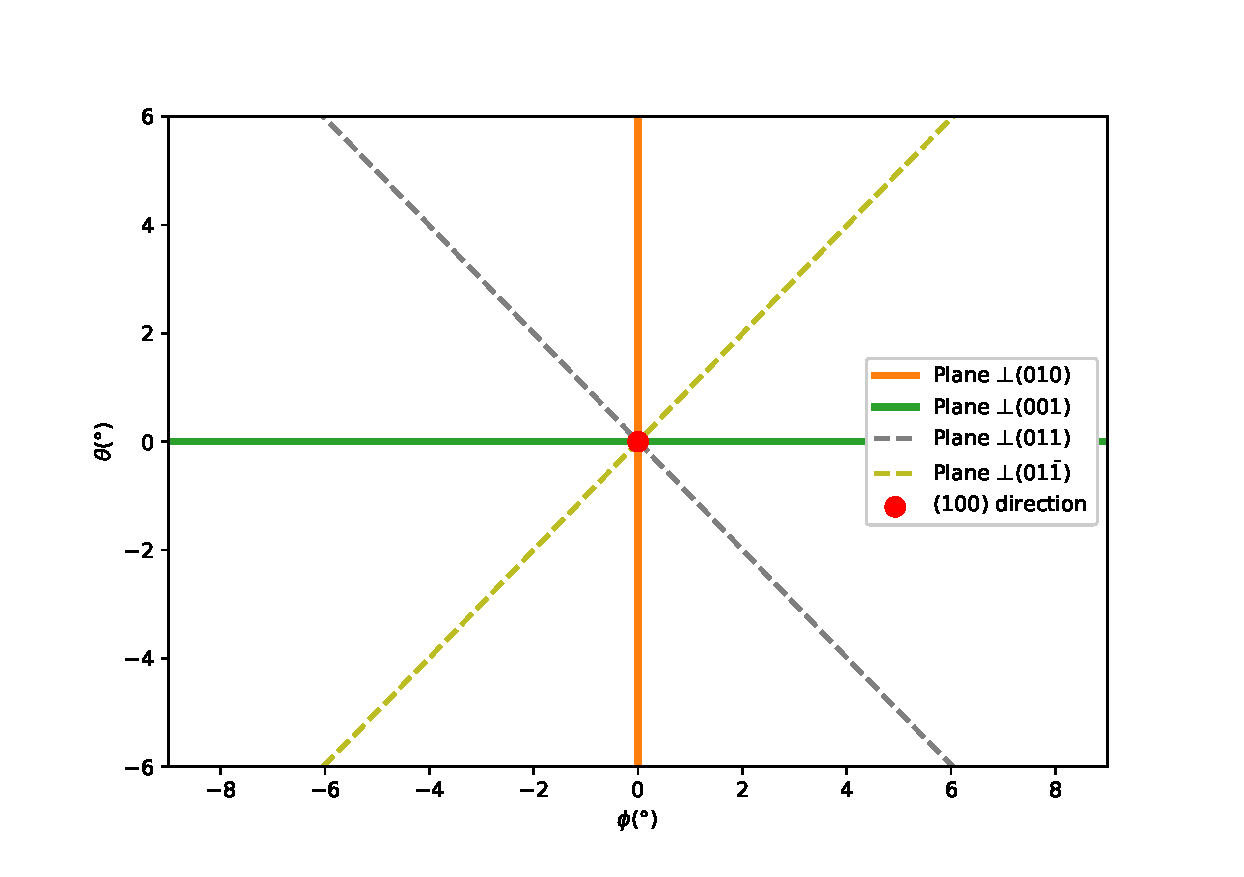
\includegraphics[width=0.4\textwidth]{map_zoom.eps}}
  \caption{a) 
Zoom on the $\langle 100 \rangle$ direction. 
 }
\end{figure}

Fig. \ref{Map} shows the NV Photoluminescence as a function of magnetic field direction, referenced by azimuthal and polar angles $(\phi, \theta)$. The PL is seen to drop for particular values of the angle. The symmetric pattern suggests that the diamond cristalline main directions play a role. Because of the anisotropy of the NV center, see \ref{Cristallo}, the NV PL drop can indeed be a signature of the cristal direction.
The drop of the PL along the cristal axis was already observed by many groups. LUKIN, HEMMER, BUDKER. JARMOLA. OORT
\cite{van_oort_optically_1991, van_oort_cross-relaxation_1989, armstrong_nvnv_2010, jarmola_longitudinal_2015, akhmedzhanov_microwave-free_2017, akhmedzhanov_magnetometry_2019, holliday_optical_1989, choi_depolarization_2017}

Charge transfer processes : 

IONISATION
2 photon Photoionisation from NV- to NV0.
OR 
Tunneling (Manson/Degen) : NV- excited state ionizes via tunneling of electrons to Ns+.

RECHARGING  : 
NV0+N0-> NV-+N+ (in the dark). 
It can occur via tunneling of electrons among closely packed NVs. 

Each of the lines is very well approximated by a Gaussian curve.


\begin{figure}[!ht]
  \centering{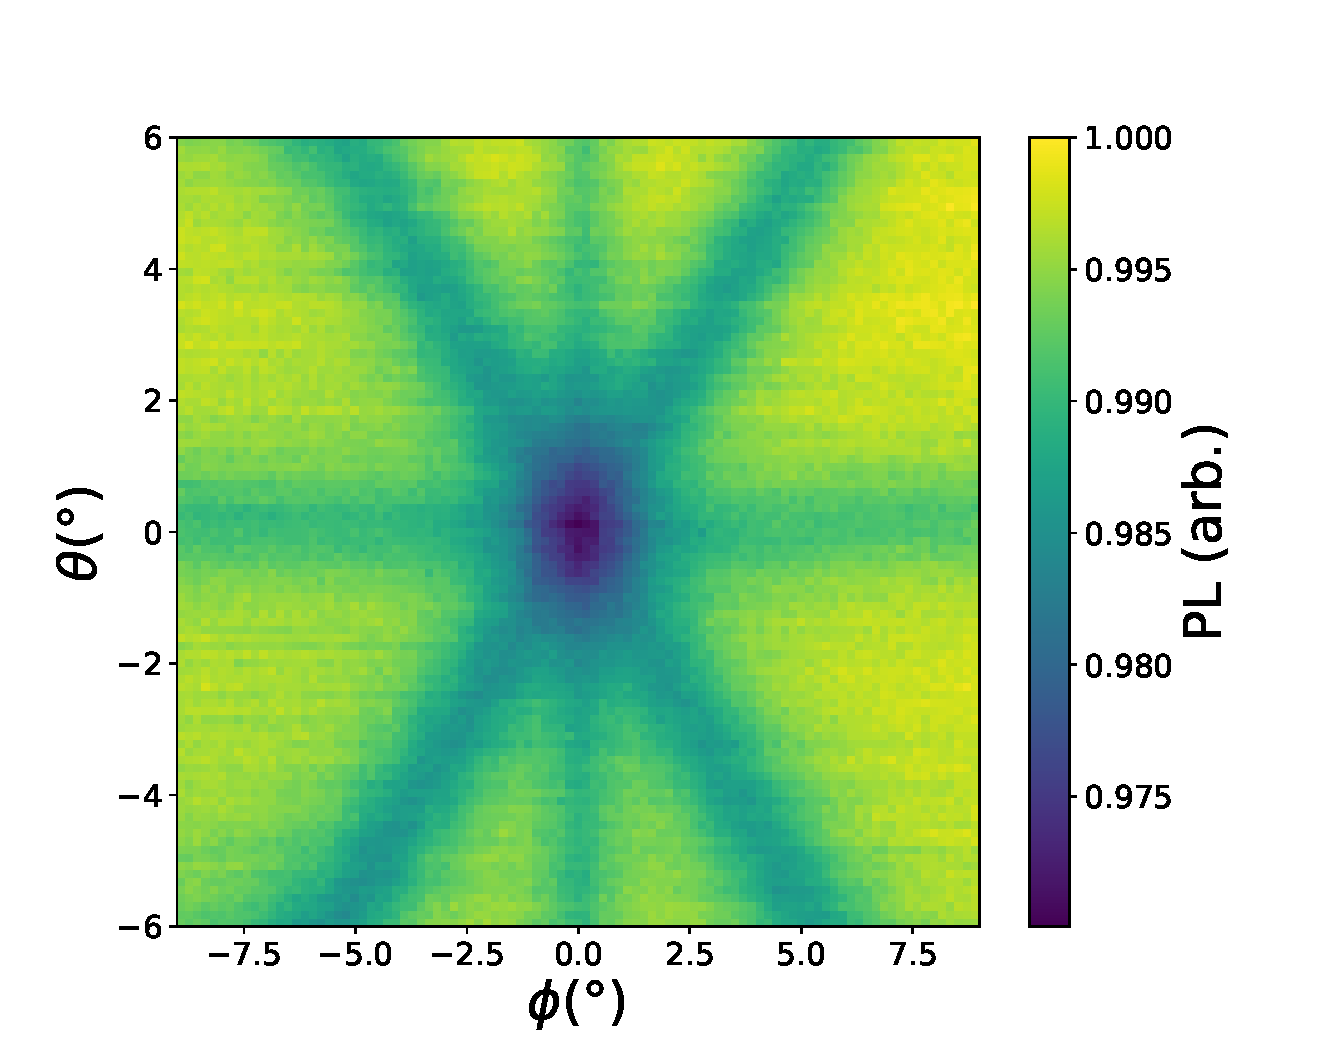
\includegraphics[width=0.40\textwidth]{Carte.eps}}
  \caption{a) 
NV Photoluminescence as a function of magnetic field direction, referenced by azimuthal and polar angles $(\phi, \theta)$.  }\label{Map}
\end{figure}

Fig.~\ref{T1} shows measurements of the $T_1$/ Tunneling is strong in the presence of nitrogen impurities. 
To remove this effect, we apply a microwave....

\begin{figure}[!ht]
  \centering{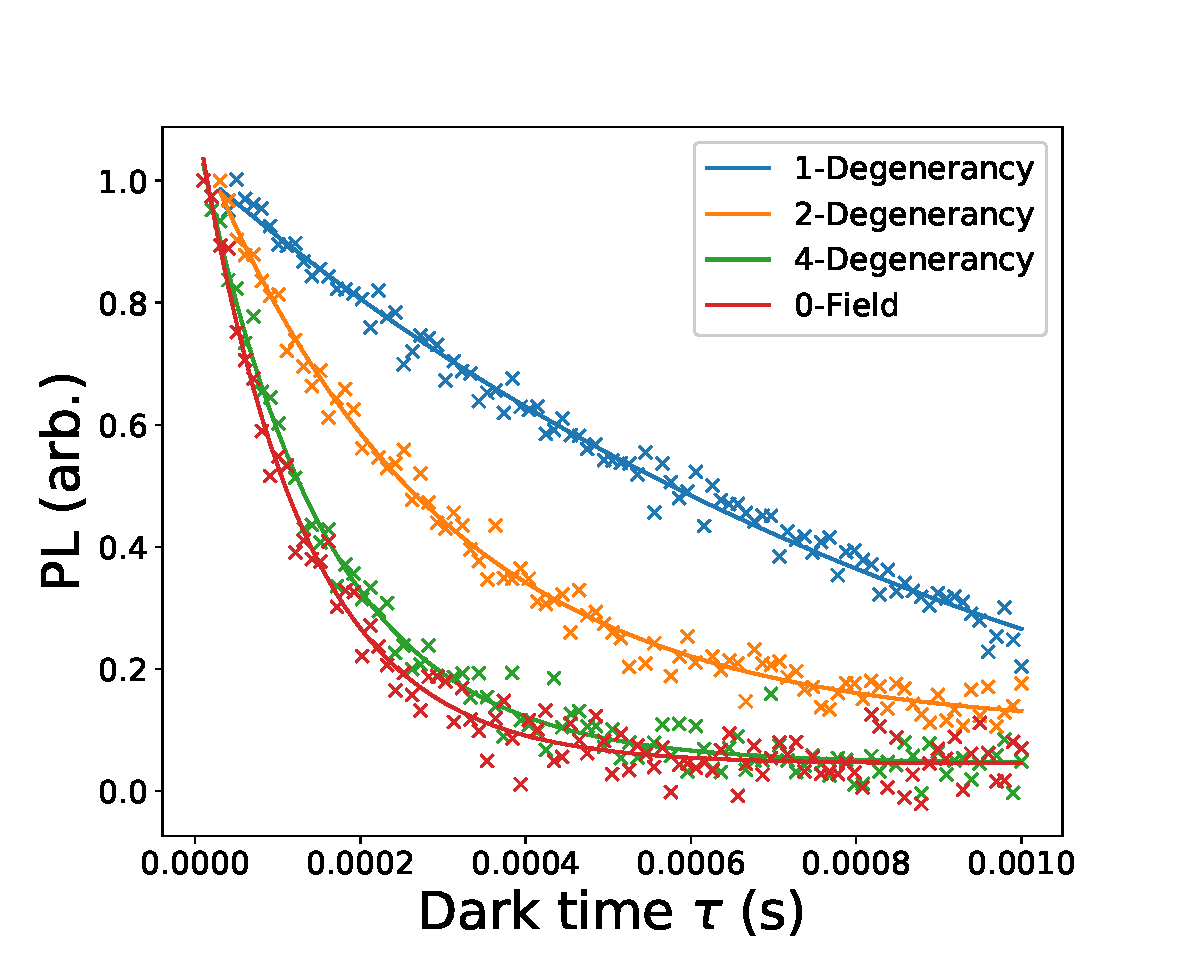
\includegraphics[width=0.40\textwidth]{T_1.eps}}
  \caption{a) 
Lifetime saturation theory
 }\label{T1}
\end{figure}


\begin{figure}[!ht]
  \centering \scalebox{0.5}{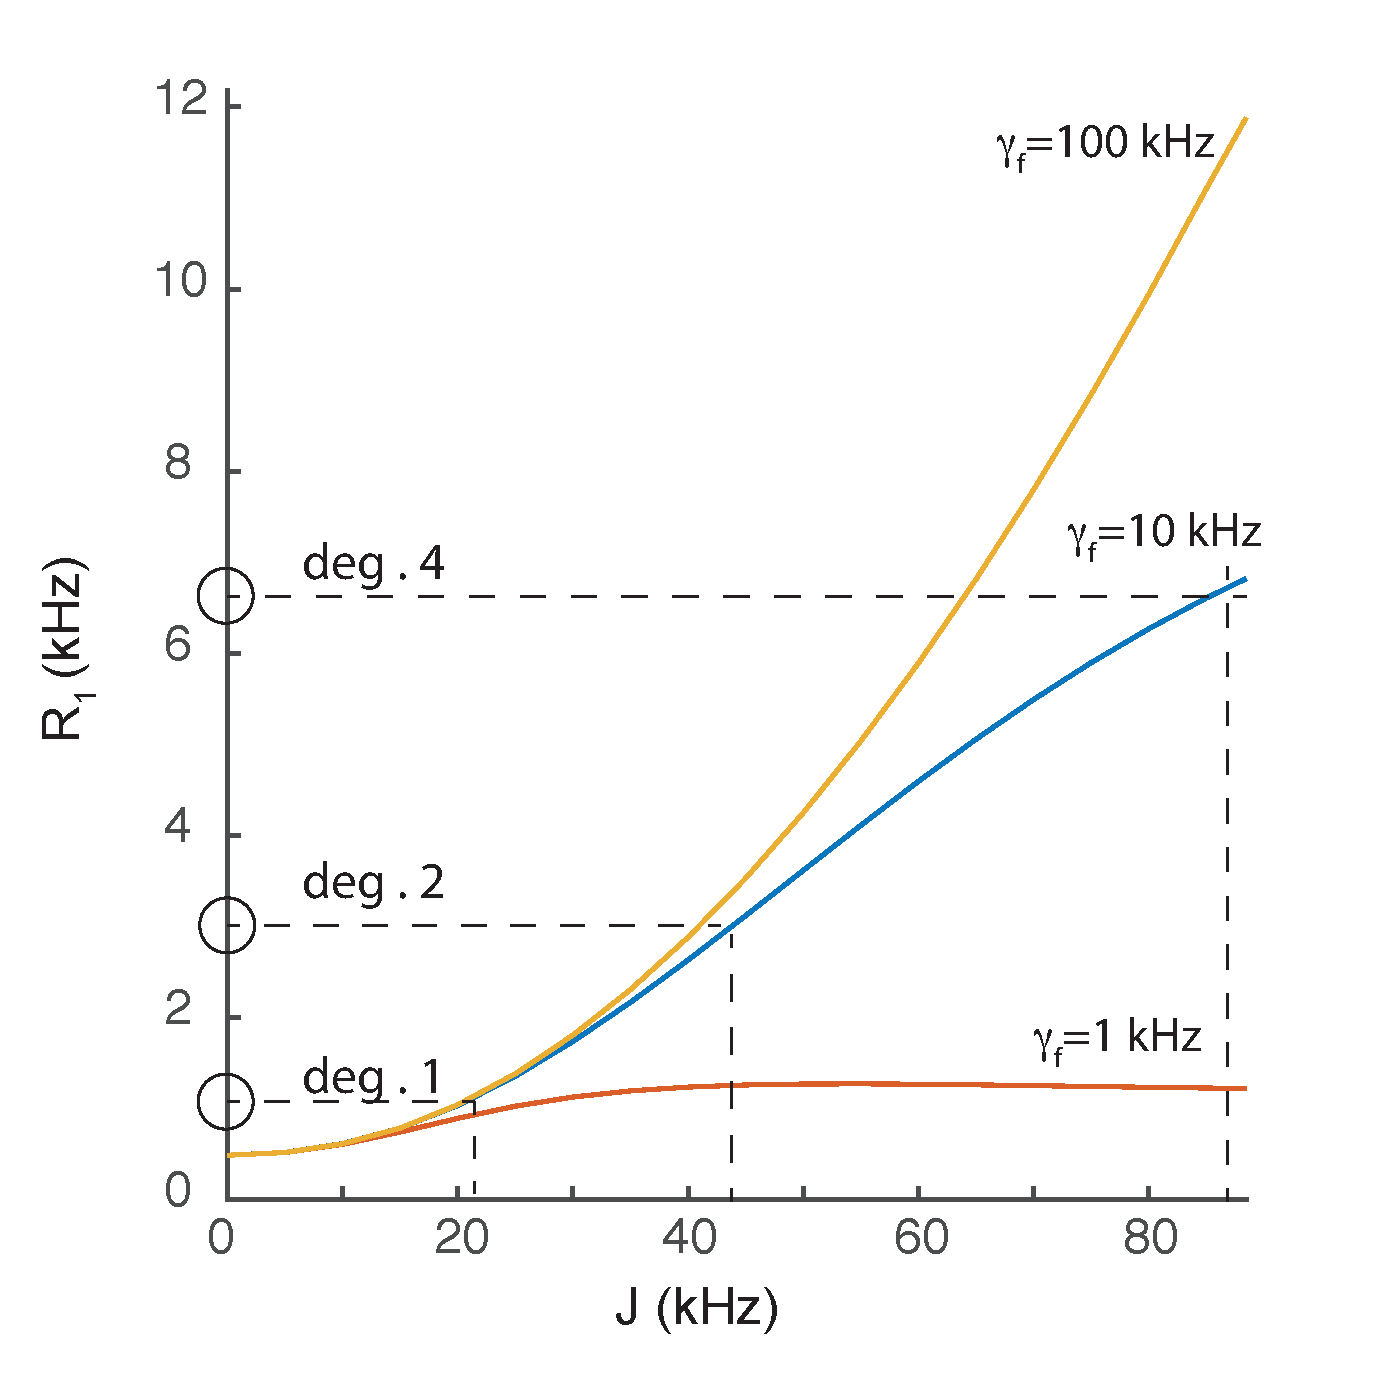
\includegraphics{R1_vs_J.pdf}}
  \caption{a) 
Lifetime saturation theory
 }
\end{figure}


\begin{figure}[!ht]
  \centering \scalebox{0.4}{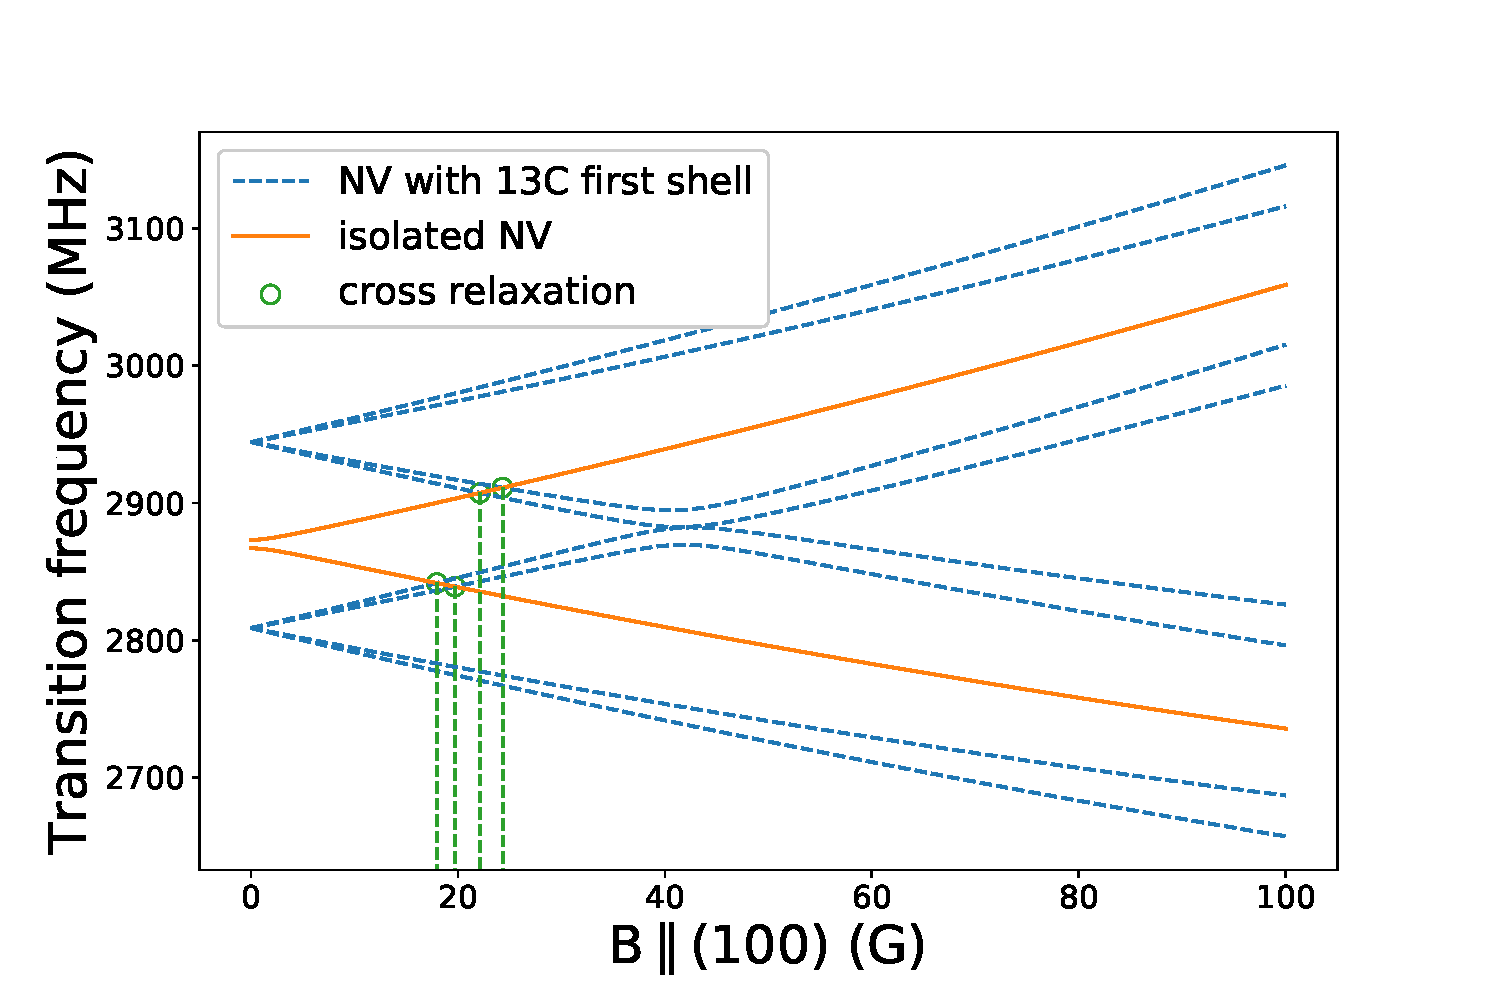
\includegraphics{13C_transitions.eps}}
  \caption{Transitions of NV-13C and NV.
 }
\end{figure}

\begin{figure}[!ht]
  \centering \scalebox{0.5}{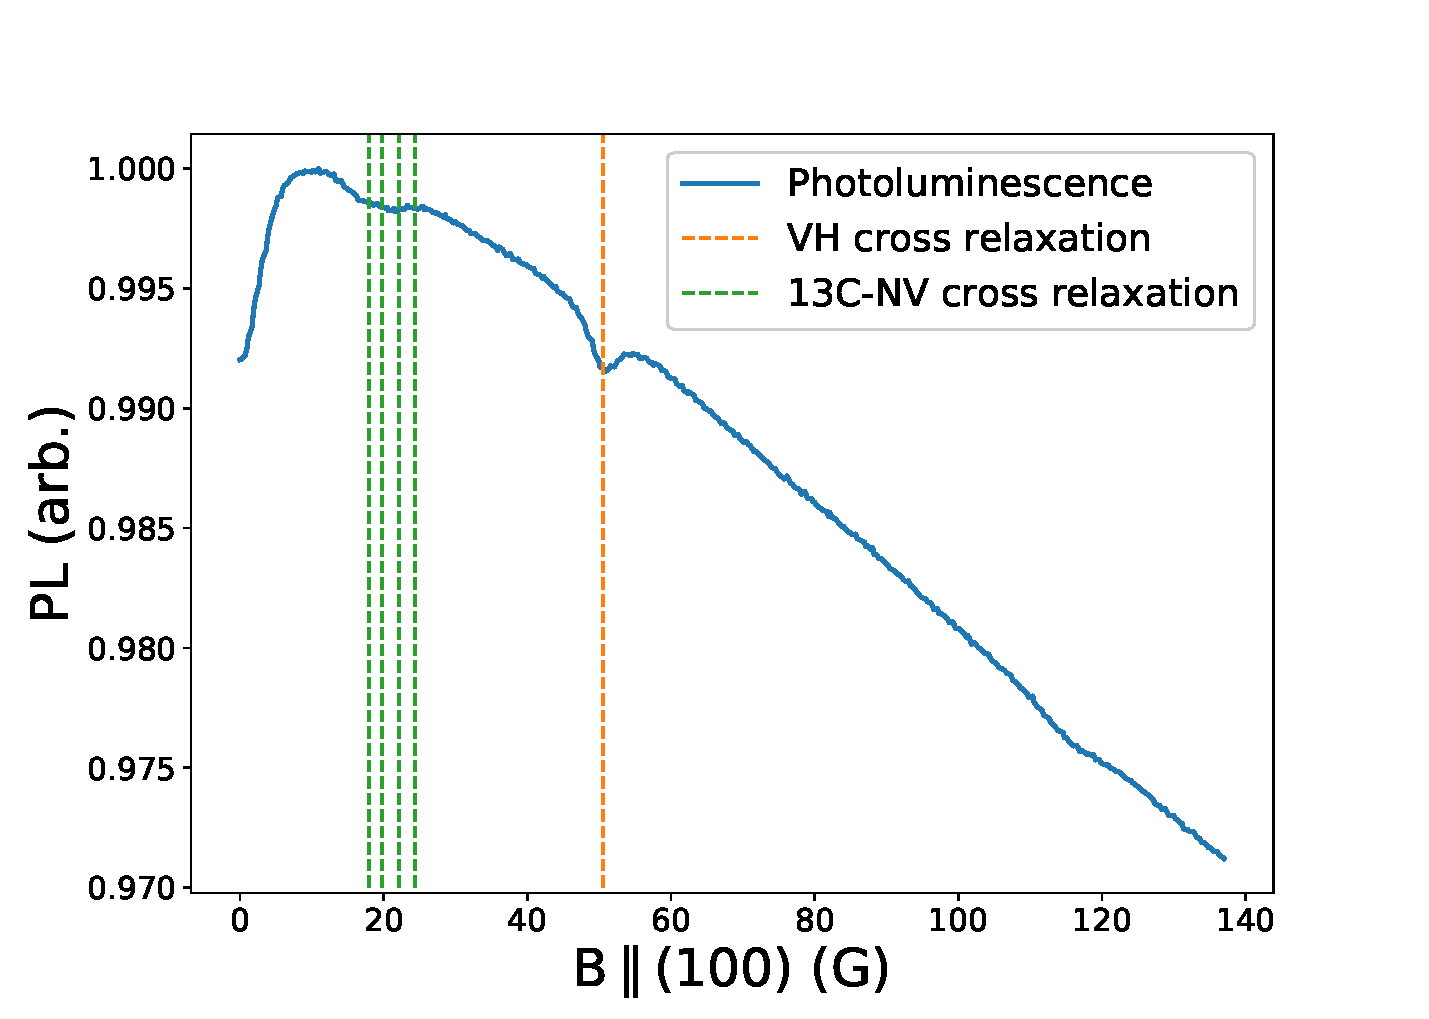
\includegraphics{rose_10V_13C.eps}}
  \caption{NV Photoluminescence as a function of a magnetic field scanned along the 100 direction. 
 }
\end{figure}

Two peaks cannot be explained. 

Hypotheses that did not work.


$NV^0, P1, 13C$ other shells, NVN (H3) center (diamagnetic in ground state), paramagnetic only in excited state but requires UV light. 
No other species were observed in the optical spectrum or EPR. 












\section*{acknowledgements}
We would like to thank Neil Manson and ... for fruitful discussions. 
GH acknowledges funding by the French National Research Agency (ANR) through the T-ERC project QUOVADIS. 

\bibliography{Biblio_dbl_quantum}



\end{document}